%%%%%%%%%%%%%%%%%%%%%%%%%%%%%%%%%%%%%%%%%
% Thin Sectioned Essay
% LaTeX Template
% Version 1.0 (3/8/13)
%
% This template has been downloaded from:
% http://www.LaTeXTemplates.com
%
% Original Author:
% Nicolas Diaz (nsdiaz@uc.cl) with extensive modifications by:
% Vel (vel@latextemplates.com)
%
% License:
% CC BY-NC-SA 3.0 (http://creativecommons.org/licenses/by-nc-sa/3.0/)
%
%%%%%%%%%%%%%%%%%%%%%%%%%%%%%%%%%%%%%%%%%

%----------------------------------------------------------------------------------------
%	PACKAGES AND OTHER DOCUMENT CONFIGURATIONS
%----------------------------------------------------------------------------------------

\documentclass[a4paper, 11pt]{article} % Font size (can be 10pt, 11pt or 12pt) and paper size (remove a4paper for US letter paper)

\usepackage[protrusion=true,expansion=true]{microtype} % Better typography
\usepackage{graphicx} % Required for including pictures
\usepackage{wrapfig} % Allows in-line images

\usepackage{float}   % plot images
\usepackage{subfig}  % plot images
\usepackage{listings}
\usepackage{algorithm} % for algorithm
\usepackage{algorithmic}
\usepackage{leftidx}
\usepackage{amsmath}
\usepackage{minted}
\usepackage{geometry}
\usepackage{relsize}

\DeclareMathOperator*{\argmin}{argmin}
\newcommand*{\argminl}{\argmin\limits}

\usepackage{mathpazo} % Use the Palatino font
\usepackage[T1]{fontenc} % Required for accented characters
\linespread{1.05} % Change line spacing here, Palatino benefits from a slight increase by default

\makeatletter
\renewcommand\@biblabel[1]{\textbf{#1.}} % Change the square brackets for each bibliography item from '[1]' to '1.'
\renewcommand{\@listI}{\itemsep=0pt} % Reduce the space between items in the itemize and enumerate environments and the bibliography

\renewcommand{\maketitle}{ % Customize the title - do not edit title and author name here, see the TITLE block below
\begin{flushright} % Right align
{\LARGE\@title} % Increase the font size of the title

\vspace{50pt} % Some vertical space between the title and author name

{\large\@author} % Author name
\\\@date % Date

\vspace{40pt} % Some vertical space between the author block and abstract
\end{flushright}
}

%----------------------------------------------------------------------------------------
%	TITLE

%----------------------------------------------------------------------------------------

\title{\textbf{Introduction to Face Detection}\\ % Title
A implementation which base on AdaBoost} % Subtitle

\author{\textsc{ZiJian Liu} % Author
\\{\textit{jasonleaster.github.io}}
\\{\textit{XiangTan University}}} % Institution

\date{\today} % Date

%----------------------------------------------------------------------------------------

\begin{document}

\maketitle % Print the title section

%----------------------------------------------------------------------------------------
%	ABSTRACT AND KEYWORDS
%----------------------------------------------------------------------------------------

%\renewcommand{\abstractname}{Summary} % Uncomment to change the name of the abstract to something else

\begin{abstract}
    We are going to introduce a method which will help us to do face detection. The idea of this system are arised by viola. In this paper, I also contribute some scheme for optimaization.
    Some face detection applications are based on nerual network but it may not be friendly to construct a nerual network. The detection system in this paper are useful and simple enough to be implemented. Data dirven application cost a lot of time, I use a concurrent framework to accelerate the training process. The time of extracting features from original images can be shorten obviously. The key point in this system is using AdaBoost to select and combine some weak classifier into a strong classifier. Finally, I demonstrate some test result of the our face detection system.

\end{abstract}

\hspace*{3,6mm}\textit{Keywords:} Face Detection, AdaBoost, Haar Feature, Machine Learning % Keywords

\vspace{30pt} % Some vertical space between the abstract and first section

\vspace*{\fill}
\begin{center}
    \textit{Version 1.2\\All Right Reserved}
\end{center}
\vspace*{\fill}
%----------------------------------------------------------------------------------------

%	ESSAY BODY
%----------------------------------------------------------------------------------------
\clearpage
\tableofcontents

\clearpage

\section{Preparation}

All training images get from MIT and CMU library and all program written by Python. So you may have to install Python into your operating system. I just use basic Python library like numpy, matplotlib, os and pylab. We don't need OpenCV. We are doing the same great thing. I use five section to introduce this project. Integrated image, Haar features, AdaBoost and the test module.

\begin{figure}[H]
    \centering
    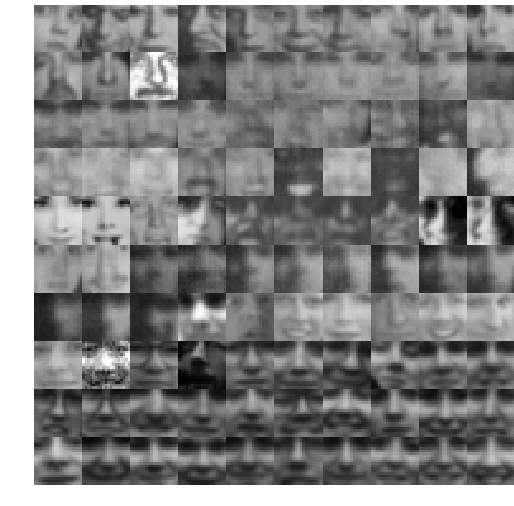
\includegraphics[width=0.38\textwidth]{../figure/combinedImage.jpg}
    \label{fig:combinedImage}
    \caption{Samples from the training set}
\end{figure}

The most application of Machine Learning are data driven. So, you may have a good workstation or PC to run the system. Otherwise, it will cost your a lot of time to training the model. 

%Don't panic :) All I have done is on my PC (Linux/Memory=4G CPU=Intel(R) core(TM) i5-3210M 2.5GHz )

To elimilate the influence of lights from environments, we should pre-process the images and normalize them.

    \begin{equation}
        \mathlarger{
        \mathlarger{
        \centering
        I(x,y) = \tfrac{I^{ori}_{x,y} - \mu}{\sqrt{\tfrac{1}{M*N} \sum_{i = 1}^{N}\sum_{j = 1}^{M} (I^{ori}_{i,j} - \mu)^{2} }}
        }
        }
        \label{equ:normalization}
    \end{equation}

    where $\mu$ is the mean value if the initial image which's size is M-row x N-col. In our training set, the size of image is 19x19 and all images are black and white. The training set contains about 2429 face images and 4548 non-face images.

    The denominator of the equation ~\ref{equ:normalization} is the standard deviation of the pixel intensity values. $I^{ori}$ means the original image in the training set. $I(x, y)$ represent the pixel at x-row, y-col in the image which is after processing.
    

\clearpage
%------------------------------------------------


\section{Integral image}
The first step of the Viola-Jones \cite{RobustRealTimeFaceDetection, RobustRealTimeObjectDetection} face detection algorithm is to turn the input image into an integral image. It's easy to do this job something like integration.

\begin{equation}
    \centering
    ii = \iint_{}^{} i(x', y')
    \label{equ:integralImage}
\end{equation}

%\begin{figure}[H]
%    \centering
%    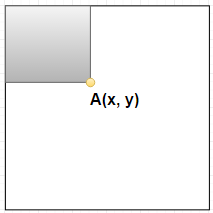
\includegraphics[height=2.in, width=2.in]{../figure/ii_demo.png}
%    \caption{ The value of the integral image at point (x, y) is the sum of all the pixels above and to the left.}
%\end{figure}


 $ii$ is the integral image and the $i$ represent as the original image. Here is a demonstration in a normal image.

     \begin{figure}[H]
        \centering
        \begin{minipage}[H]{0.3\linewidth}
        \centering
        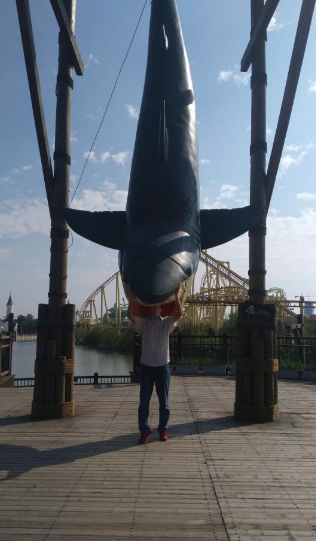
\includegraphics[height=2.5in, width=\linewidth]{../figure/bigshark.png}
        \end{minipage}
        \begin{minipage}[H]{0.3\linewidth}
        \centering
        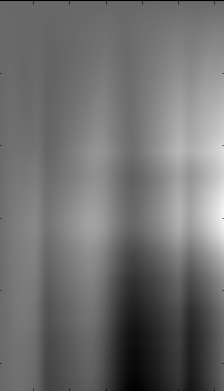
\includegraphics[height=2.5in, width=\linewidth]{../figure/integralImageOfBigShark.png}
        \end{minipage}
        \label{fig:normalImage}
        \caption{ The left side is a normal image in our daily life. The right side is the integral image of the origianl left side image.}
    \end{figure}

    The following figure are one of the sample face and it's integral image.
    \begin{figure}[H]
        \centering
        \begin{minipage}[t]{0.25\linewidth}
        \centering
        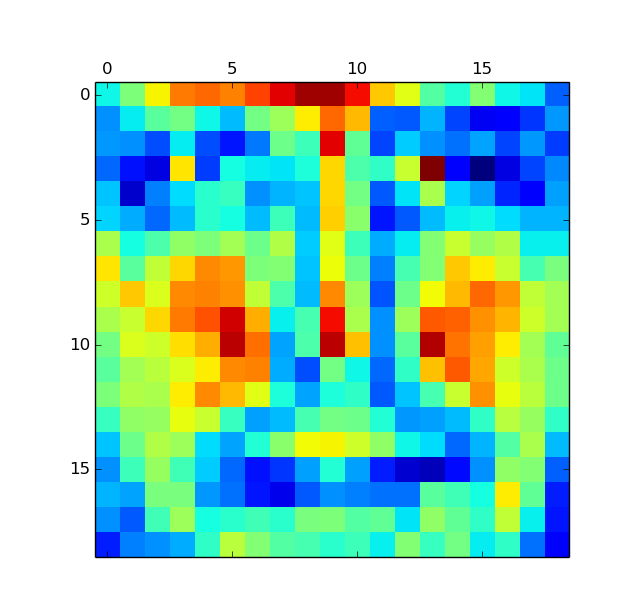
\includegraphics[height = 1.0in, width= 1.0in]{../figure/face00001.png}
        \end{minipage}
        \begin{minipage}[t]{0.25\linewidth}
        \centering
        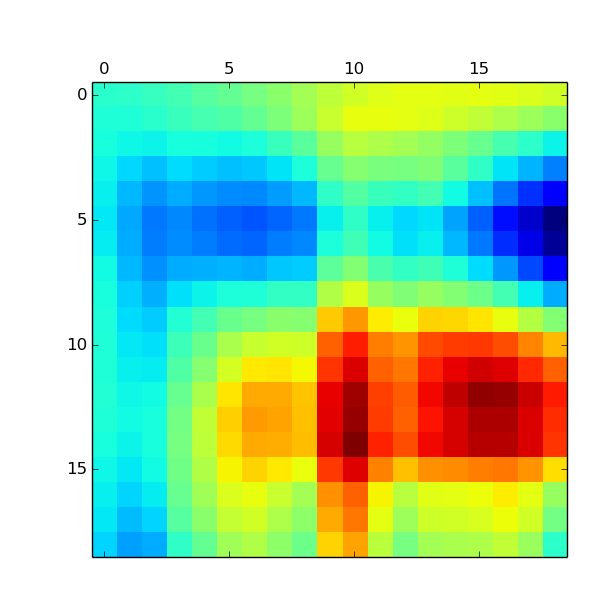
\includegraphics[height = 1.0in, width= 1.0in]{../figure/integralImageOfFace00001.png}
        \end{minipage}
        \label{fig:integralImageFace}
        \caption{Image on the left is a training sample(face00001.pgm) which is show by Python matplotlib and the right side is the corresponding integral image. Here is a check point if you want to determine whether your implementation is right or wrong.}

    \end{figure}

    What does the integral image use for ?
    This allow for the calculation of the sum of all pixels inside any given rectangel using only for values -- the boundary point of that rectangel.

    
%------------------------------------------------

\clearpage
\section{Haar Features}
    When we zoom the image we can find the image constructed with a lots of block(pixels). They like rectangles with different pattern. That's the essential of how the digital images are constructed. If you have the basical understanding of digital image, you must know that the digital image are constructed with a lots of pixels which's value come from 0 to 255.\\

    The detection system are based on the value of simple features but not using the pixels directly. The reason given by Voila is that "features can act to encode ad-hoc domain knowlege that is difficult to learn using a finite quantity of training data."\\

    The features used in the system are haar-liked features \cite{RobustRealTimeFaceDetection}, which is similary with haar wavelets. There are other feature like LIF(Local Invariant Feature) \cite{LocalInvariantFeatureDetectors} . But we didn't use it for the limitation of time.\\

\textbf{From my perspective, it's a trick to raise demention of samples.}\\


    We used four different pattern in our implementation. They are shown in the folloing figure.

    \begin{figure}[H]
        \centering
        \subfloat[Type I]
        {
            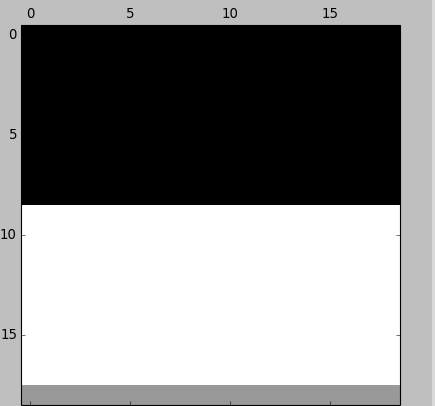
\includegraphics[height = 0.7in, width = 0.7in ]{../figure/featureTypeI.png}
        }
        \subfloat[Type II]
        {
            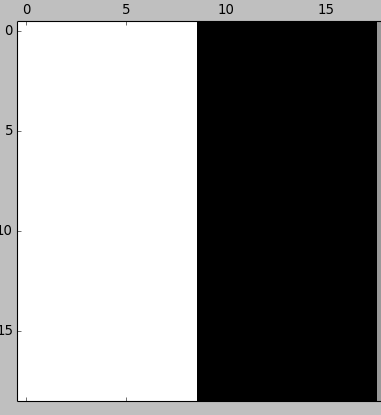
\includegraphics[height = 0.7in, width = 0.7in ]{../figure/featureTypeII.png}
        }
        \subfloat[Type III]
        {
            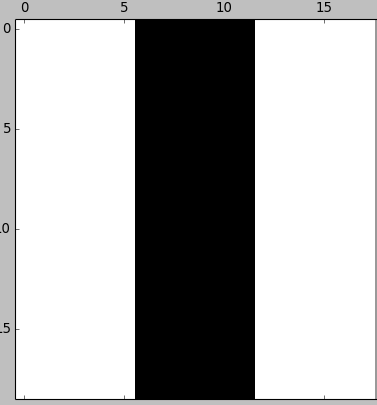
\includegraphics[height = 0.7in, width = 0.7in]{../figure/featureTypeIII.png}
        }
        \subfloat[Type IV]
        {
            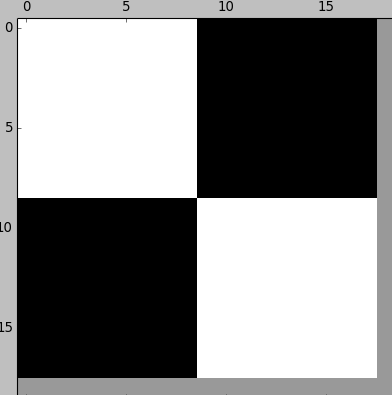
\includegraphics[height = 0.7in, width = 0.7in]{../figure/featureTypeIV.png}
        }
        \label{fig:differentHaarFeature}
        \caption{Four different types of Haar features.}
    \end{figure}

    Viola-Jones use 24*24 detetor window. Instead, I use 19*19 detector. Becasue my the size of my training set images are 19*19. Diffient size of window have different number of features. That's all right.\\
    The value of each features are calculated by sum of pixelsa which lie within the white rectangles are subtracked from the sum of pixels in the grey rectangles.\\
    In my implementation, features are represented as list like this "["II", x, y, w, h]". This means that the type of the selected feature is "II". It start point is (x, y). The width of the rectangle is w and the h is the height of the rectangle.\\
    In Voila's and others work, they used all the features within the detector window, the number of that around 160,000. It's too large and cost a lot of time to compute 16,000 for every subwindow. In my implementation, I optimalized the feature generator which will drop out some feature and make the computation process more faster. I only used about 13,000 features to build our detection system.

\clearpage
\section{Weak Classifier}
Weak classifier\cite{ImprovedBoostingAlgorithmUsingConfidenceRatedPredictors} is a type of classifier which can not classify all samples correctly. But they also do good job on classification. A good weak classifier can classify samples with the correct rate over than 50\%. Yes, it can be 99\% or 51\%. It just better than guess randomly.

    \begin{algorithm}[H]
        \caption{Simple weak classifier}
        \textbf{Input}: A set of feature responses $ \{ \leftidx{f}{_{j} (x1)}, ..., \leftidx{f}{_{j} (xn)} \} $ extracted by appliying the feature $\leftidx{f}{_{j}} $ to each training sample $\leftidx{x}{_{i}} $ and associatd labels \{ $\leftidx{y}{_{1}}, ..., \leftidx{y}{_{n}}$ \}. A set of non-negative weights \{ $\leftidx{w}{_{1}}, ..., \leftidx{w}{_{n}}$ \} \\

        \textbf{Output}: $\theta$ is a threshold value. Attention! p $\in \{-1, +1\} $is a direction value. When the mean value of positive samples smaller than the mean value of negative samples, the direction value p is 1. otherwise, it's -1.

        \begin{equation}
            g(\leftidx{f}{_{i}} ; p; \theta ) = 
            \begin{cases}
                & \text{1 if } p \leftidx{f}{_{j} (x)} < p \theta \\
                & \text{0 if } otherwise
            \end{cases}
            \label{equ:weakClassifier}
        \end{equation}

        e is the error rate of the result of classification by this weak classifier g. \textbf{e must be smaller than 0.5}\\

        \textbf{Steps of algorithm} \\

        $\bullet$  Compute the weighted mean of the positive samples and negative samples.
        \begin{equation}
            \mu_{P} = \tfrac{\sum_{i = 1}^{n} w_{i} f_{j}   (x_{i}) y_{i}}
                                        {\sum_{i=1}^{n} w_{i} y_{i}},
            \mu_{N} = \tfrac{\sum_{i = 1}^{n} w_{i} f_{j}   (x_{i}) y_{i}}
                                        {\sum_{i=1}^{n} w_{i} y_{i}}
        \end{equation}

        $\bullet$ Set the threshold to $\theta = \tfrac{1}{2} (\mu_{P} + \mu_{N})$ .\\

        $\bullet$ Compute the error associatd with the two possible values of the direction.

        \begin{equation}
            \varepsilon_{-1} = \sum_{i = 1}^{n} w_{i} \left | y_{i} - g(f_{i}(x_{i}); -1; \theta) \right |
        \end{equation}

        \begin{equation}
            \varepsilon_{+1} = \sum_{i = 1}^{n} w_{i} \left | y_{i} - g(f_{i}(x_{i}); +1; \theta) \right |
        \end{equation}

        $\bullet$ Set $p^{*} = \argminl_{p \in \{-1, +1\}} \varepsilon_{p^{*}}$
    \end{algorithm}

    \begin{figure}[H]
        \centering
        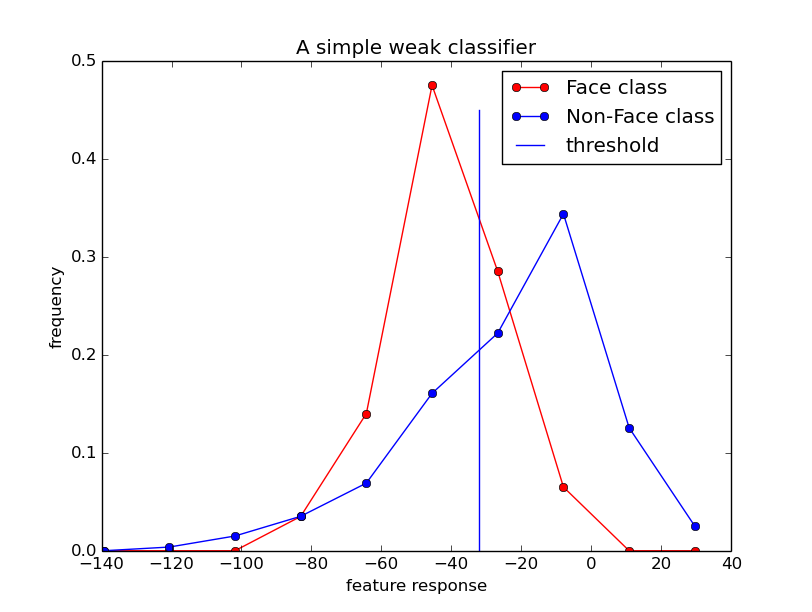
\includegraphics[width = 0.7\linewidth]{../figure/simpleClassifier.png}
        \label{fig:simpleWeakClassifier}
        \caption{A simple weak classifier. The red curve is the histogram of face class and the blue curve is the histogram of Non-Face class.}
    \end{figure}

    The figure above there show what a good weak classifier look like. The more overlap between the two histogram and the more bad the result of classification by any possible threshold. It's important to know that the direction of classification depend on the error rate of two type of sample set.

    More detail, I show a pieace of code in the detection system. Reader can understand what I have done more deeply.

    \begin{minted}{python}
    for direction in [-1, 1]:
        errorRate = 0.
        for i in range(self.SampleNum):
            if self._Mat[d][i] *direction < threshold * direction:
                output[i] = LABEL_POSITIVE # positive label +1
            else:
                output[i] = LABEL_NEGATIVE # positive label -1

            if output[i] != self._Tag[i]:
                errorRate += self.weight[i]

        if errorRate < minErrRate:
            minErrRate    = errorRate
            bestDirection = direction

    return minErrRate, threshold, bestDirection
    \end{minted}

\clearpage
\section{AdaBoost}
What's the next step? We have got the weak classifier. Let's use it to construct a strong classifier by boosting \cite{BIASVARIANCEANDARCINGCLASSIFIERS}.

    With window size of 19*19 pixels of the detector, there are huge number of features in the window. Every feature is a classifier. It also means that there are a lots of weakclassifier. There is a problem that which classifier we should use to do the job about classification. \\

    There may have other solution like SVM, nerual network and other machine learning algorithm. In this paper, we try to solve this problem by AdaBoost which is a very useful and efficient algorithm to do classification.

    \begin{algorithm}
        \caption{AdaBoost}

        \textbf{Input:} Give sample $(x_{1}, y_{1}), ..., (x_{n},y_{n})$ where $y \in \{-1, +1\}$\\

        \textbf{Output:} G is the strong classifier which produce by this algorithm.\\

        \textbf{Steps of algorithm}\\

        $\bullet$ Initialize weights $w_{1,i} = \tfrac{1}{2m}, \tfrac{1}{2l}$ for $y_{i} = 0, 1$ respectively.\\

        $\bullet$ For t = 1, ..., T
                \begin{enumerate}
                    \item normalize the weight $w_{t, i} = \tfrac{w_{t, i}}{\sum_{i = 1}^{n} w_{t, i}}$
                    \item select the best weak classifier with respect to the weighted error rate.
                    \item Define $g_{t}(x) = g(x, f_{t}, p_{t}, \theta_{t})$ where $f_{t}, p_{t}, and \theta_{t}$ are the minimizers of $\varepsilon_{t}$

                    \item Update the weights
                \end{enumerate}

        $\bullet$ The final strong classifier is:\\
            \begin{equation}
            G(x) = 
            \begin{cases}
                & \text{1 if } \sum_{t = 1}^{T} \alpha_{t} g_{t} (x) >= \tfrac{1}{2} \sum_{t = 1}^{T} \alpha_{t}\\
                & \text{0 if } otherwise
            \end{cases}
            \end{equation}
    \end{algorithm}

\clearpage
    Here is a demonstration that the features which are selected by AdaBoost. For presentation, there are 10 features in the following figure.

    \begin{figure}[H]
        \centering
        \subfloat[]
        {
            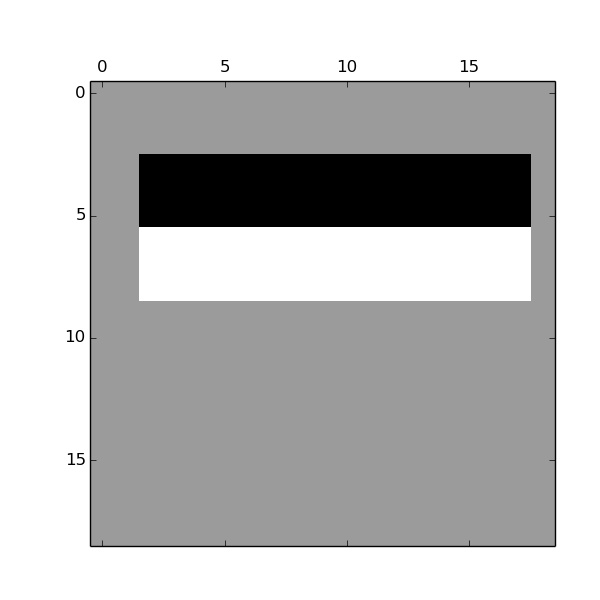
\includegraphics[height = 0.7in, width = 0.7in ]{../figure/feature_0.jpg}
        }
        \subfloat[]
        {
            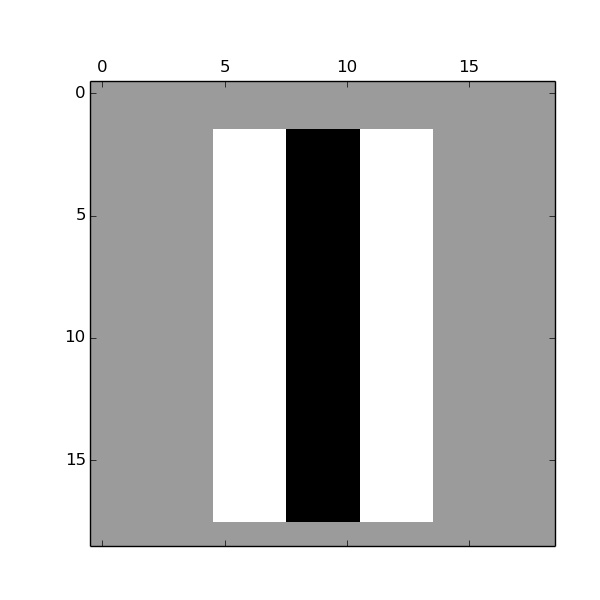
\includegraphics[height = 0.7in, width = 0.7in ]{../figure/feature_1.jpg}
        }
        \subfloat[]
        {
            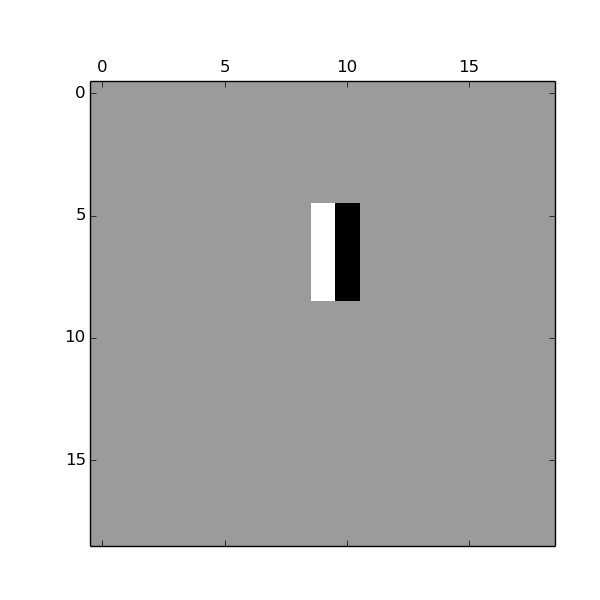
\includegraphics[height = 0.7in, width = 0.7in ]{../figure/feature_2.jpg}
        }
        \subfloat[]
        {
            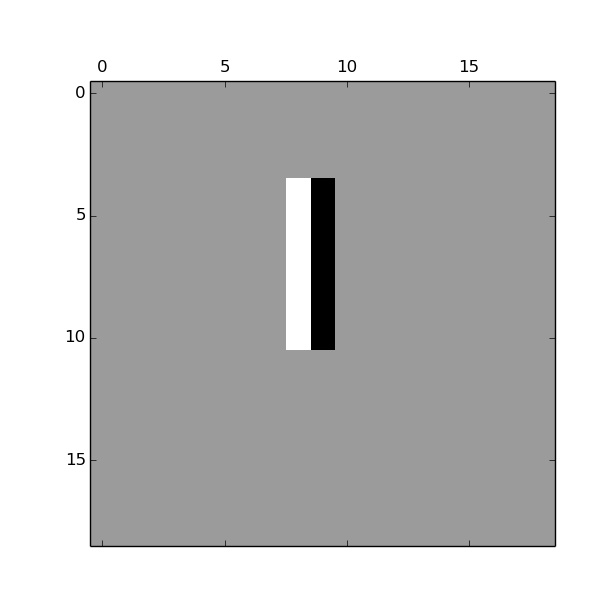
\includegraphics[height = 0.7in, width = 0.7in ]{../figure/feature_3.jpg}
        }
        \subfloat[]
        {
            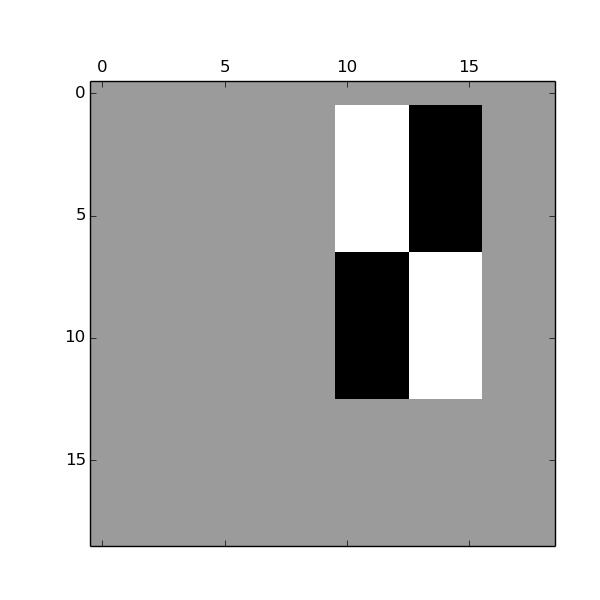
\includegraphics[height = 0.7in, width = 0.7in ]{../figure/feature_4.jpg}
        }\\
        \subfloat[]
        {
            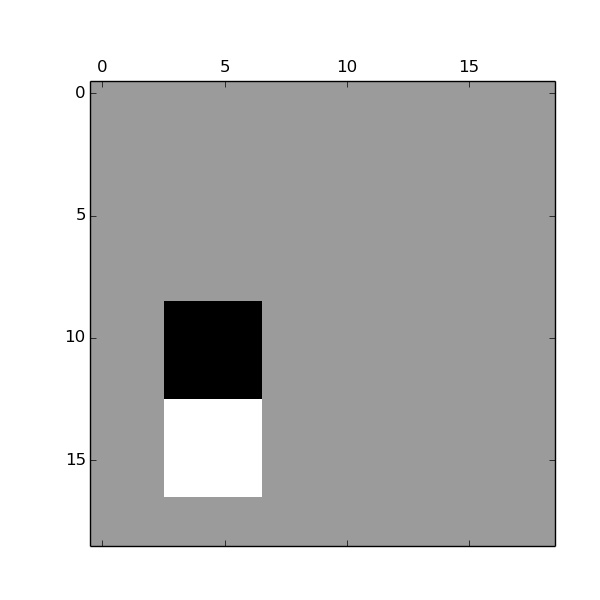
\includegraphics[height = 0.7in, width = 0.7in ]{../figure/feature_5.jpg}
        }
        \subfloat[]
        {
            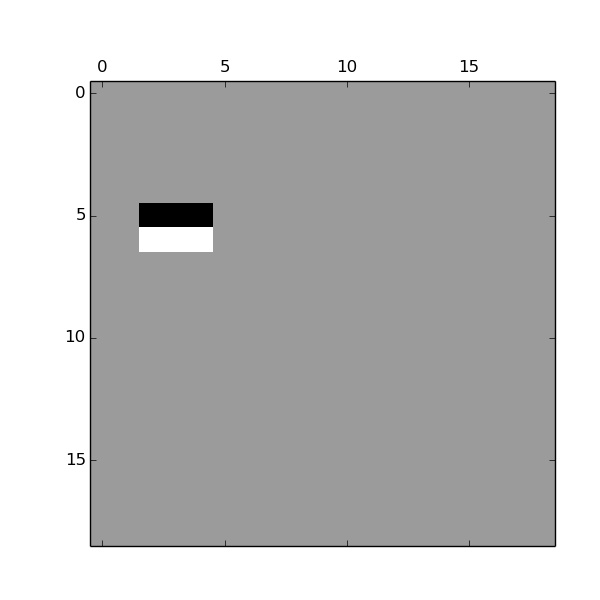
\includegraphics[height = 0.7in, width = 0.7in ]{../figure/feature_6.jpg}
        }
        \subfloat[]
        {
            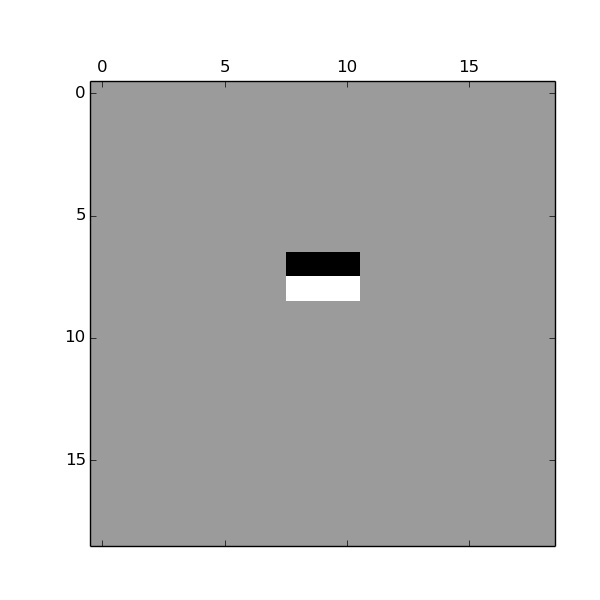
\includegraphics[height = 0.7in, width = 0.7in ]{../figure/feature_7.jpg}
        }
        \subfloat[]
        {
            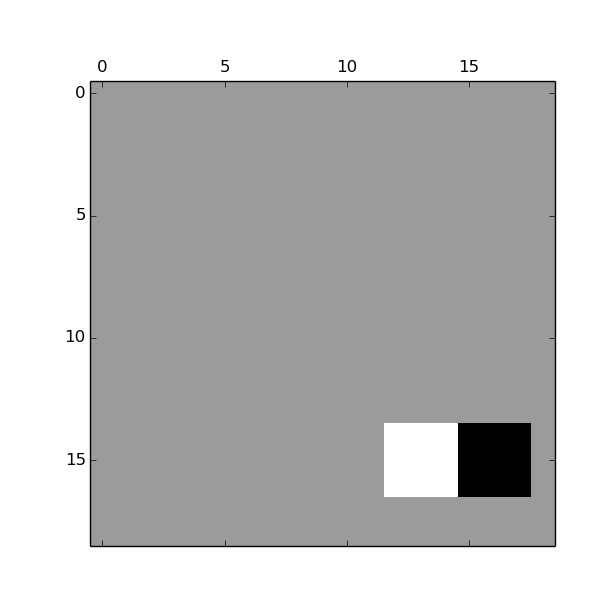
\includegraphics[height = 0.7in, width = 0.7in ]{../figure/feature_8.jpg}
        }
        \subfloat[]
        {
            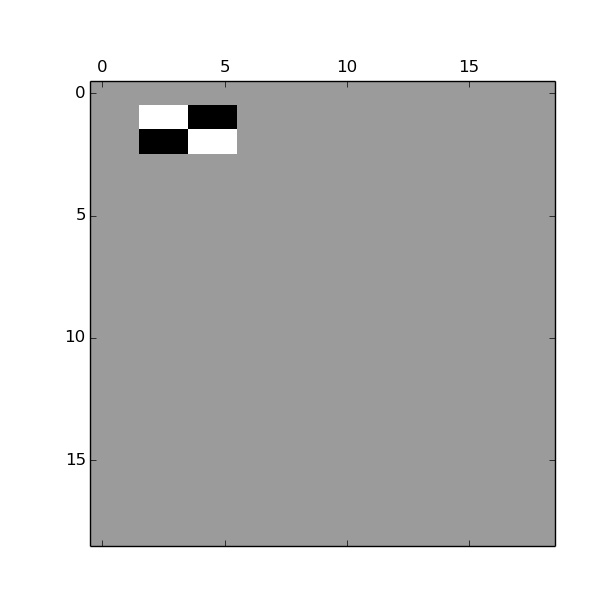
\includegraphics[height = 0.7in, width = 0.7in ]{../figure/feature_9.jpg}
        }

        \caption{Ten features selected by AdaBoost}
        \label{fig:tenWeakClassifier}
    \end{figure}

    \begin{figure}[H]
        \subfloat[boosted classifier by feature shown in figure ~\ref{fig:tenWeakClassifier}]
        {
            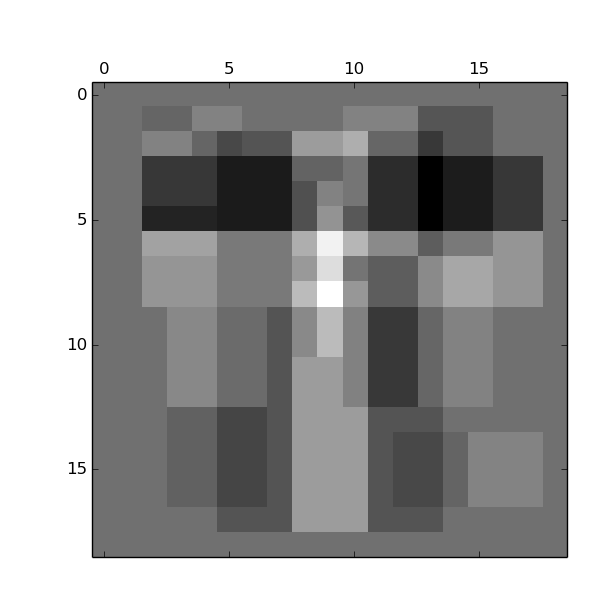
\includegraphics[height = 2.7in, width = 2.7in ]{../figure/combinedClassifierPic.png}
        }
        \subfloat[A human face from training set]
        {
            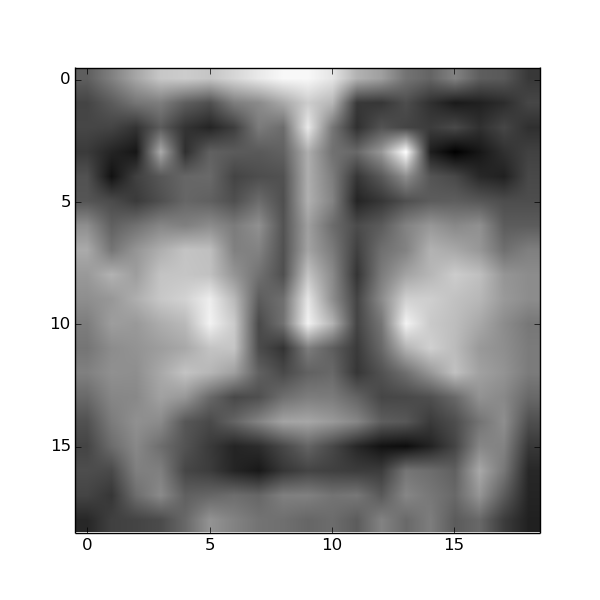
\includegraphics[height = 2.7in, width = 2.7in ]{../figure/humanFace.png}
        }
        \label{fig:float}
        \caption{The final strong classifier with boosted 10 weak classifier and human face}
    \end{figure}
    Here, I compare the final classifier image with a training sample of human face. You will find that the more final classifier image look like to human face, the better final classifier are.

    Why not use a human face image as a classifier directly?

    My answer is "Do you forget what means overfitting? "

\clearpage

Look at table ~\ref{table:finalClassifier}, I show a detail information about the final classifier. All the information are cached in local file \textit{/model/model.cache}
    \begin{table}[H]
        \centering
        \caption{Detail information about the final classifier}
        \begin{tabular}{l c c c c c c c c c c}
            \hline
            \hline
            Figure                  & 1     & 2     & 3     & 4     & 5     & 6     & 7     \\
            Feature Number          & 5287  & 13455 & 5797  & 6091  & 15360 & 1988  & 1165  \\
            $\alpha$ (Voting power) & 1.9266& 1.4872& 0.9625& 1.0217& 0.9213& 0.7948& 0.6828\\
            p (Direction)           & +1    & -1    & +1    & -1    & +1    & -1    & +1    \\
            Figure                  & 8     & 9     & 10    \\
            Feature Number          & 1214  & 7937  & 14491 \\
            $\alpha$ (Voting power) & 0.7103& 0.6336& 0.6116\\
            p (Direction)           & +1    & +1    & -1    \\
            \hline
        \end{tabular}
        \label{table:finalClassifier}
    \end{table}


    We have got the final classifier. We also know the threshold of each selected weak classifier. But what about the threshold of final classifier ? Here we should introduce some concepts which are used in the definition of the ROC-curve.

    \begin{table}[H]
        \centering
        \caption{A classifier predicts the class of a test example}
        \begin{tabular}{l c c}
            \hline
            \hline
            Label              & Predicted Class& True Class    \\
            True-Positive (tp) & Positive       & Positive      \\
            False-Positive(fp) & Positive       & Negative      \\
            True-Negative (tn) & Negative       & Negative      \\
            False-Negative(fn) & Negative       & Positive      \\
            \hline
        \end{tabular}
        \label{table:predicts}
    \end{table}

    Our target is to try our best to detect more face and avoid to mis-detect a non-face region as a face. That's something listening like quadratic programming. When we want to maximize the tpr(True-Postive Rate) and minimize the fpr(False-Negative Rate).

    \begin{equation}
        TruePostive Rate = tpr = \tfrac{n_{tp}}{n_{tp} + n_{fn}}
    \end{equation}

    \begin{equation}
        FalsePositive Rate = fpr = \tfrac{n_{fp}}{n_{tn} + n_{fp}}
    \end{equation}

    $n_{tp}$ is the number of True-Postive etc. It's not hard to understand that tpr and fpr will vary depending on the threshold applied to the final strong classifier. The ROC(Receiver operating characteristic) curve is a way to summarize this variation. It is a curve that plots fpr Vs tpr as the threshold varies from $-\infty$ to $+\infty$.\\

    Don't forget we didn't have a good threshold for our final classifier. The ROC curve help us to choose a good threshold to do classification finally.\\

    \begin{figure}[H]
        \centering
        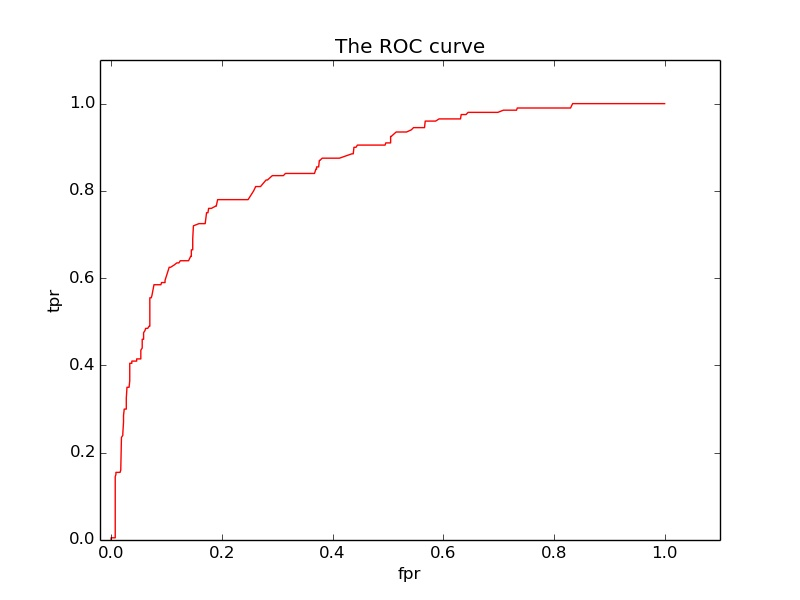
\includegraphics[height = 3.7in, width = 3.7in ]{../figure/roc.jpg}
        \caption{ROC cure computed from the images with 200 positive samples and 800 negative samples}
        \label{fig:ROC}
    \end{figure}

    With the limitation of my computer, I only used 1000 samples to training our model. If my face detection system could run on more powerful workstation, I think the result will be more beautiful.

    \begin{table}[H]
        \centering
        \caption{A classifier predicts the class of a test example}
        \begin{tabular}{l c c c c c c c}
        \hline
        \hline
        FinalThreshold  & -15.0 & -6.62     & -2.1  & 0.4       & 5.7       & 10.0\\
        tpr             & 1.0   & 0.99      & 0.81  & 0.615     & 0.005     & 0.00\\
        fpr             & 1.0   & 0.8275    & 0.27  & 0.1025    & 0.0025    & 0.00\\
        \hline
        \end{tabular}
        \label{table:selectThreshold}
    \end{table}

    We extracted some classical data from total set and table ~\ref{table:selectThreshold} show us that how the tpr and fpr will vary when the final threshold is changing. In our experiment, the final threshold is $3.1$

    \clearpage
    Here is could glance at the detail about how to compute the ROC Curve in our detection system.
    \begin{minted}{python}
    def showROC(self):
        tprs, fprs = [], []
        best_tpr, best_fpr, best_th  = 0., 1., None
        for t in numpy.arange(AB_TH_MIN, AB_TH_MAX, 0.02):
            output = self.prediction(self._Mat, t)

            Num_tp, Num_fn, Num_tn, Num_fp = 0, 0, 0, 0
            for i in range(self.SamplesNum):
                if self._Tag[i] == LABEL_POSITIVE:
                    if output[i] == LABEL_POSITIVE:
                        Num_tp += 1
                    else:
                        Num_fn += 1
                else:
                    if output[i] == LABEL_POSITIVE:
                        Num_fp += 1
                    else:
                        Num_tn += 1

            tpr = Num_tp * 1./(Num_tp + Num_fn)
            fpr = Num_fp * 1./(Num_tn + Num_fp)

            if tpr >= best_tpr and fpr <= best_fpr:
                best_tpr, best_fpr, best_th  = tpr, fpr, t
                
            tprs.append(tpr)
            fprs.append(fpr)
    \end{minted}


\clearpage
\section{Face Detection and optimaization}
\subsection{Search and detection}

    After we learnt a strong classifier.
    Now, we get the final part of the detection system. Normaly, we do search work and travel all sub-window as figure ~\ref{fig:mona} shown. Every sub-window with size 19 x 19 may contain a face image, we may have to try every sub-window, or almost every.

    \begin{figure}[H]
        \centering
        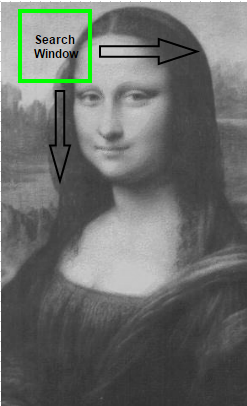
\includegraphics[height = 3.7in, width = 2.7in ]{../figure/searchWindow.png}
        \caption{Mona Lisa}
        \label{fig:mona}
    \end{figure}

    Becasue of the size of our detector is 19 x 19 and the training set image are also that size. It's very small for our daily image. It's nessesary to resize the original image into a smaller one.\\

    In our implementation, I write a function scanImgFixedWin(image, scale) which take two arguments @image and @scale. The @image is a single channel image and @scale is in (0., 1.). This function return a list of sub-window which have a face which is predicted by the AdaBoost. For convenient, the returned sub-window represent as a tuple (x, y, w, h).
(x, y) is the start point of the sub-window.  w, h are the percentage of width and height of the original image.


\clearpage
\subsection{Optimalization}

    The figure below there shown a comparision between the detection result of the ordinary detection system and the image after optimalization. You can view some overlapped rectangel in the left figure below there. And there only one rectangle with the sinle woman who is in the image.

    \begin{algorithm}
        \caption{Deduce overlapped sub-window}

        \textbf{Inout:} a set of sub-windows which are predicted as containing a human face and a threshold to determine whether the sub-window should be reduced .\\
        \textbf{Output:} set of deduced sub-windows.
        \begin{algorithmic}
        \FOR{ i from 1 to N}
            \FOR{for j from i to N}
            \STATE    overlapArea = $S_{i} \cap S_{j}$
            \STATE    totalArea   = $S_{i} \cup S_{j}$
            \STATE    overlapRate[i][j] = overlapArea / totalArea
            \ENDFOR

        \ENDFOR
        \STATE reduced = [1, ...,i, ..., N]
        \FOR{ i from 1 to N}
            \FOR{j from i+1 to N}
            \STATE  if overlapRate[i][j] > overlap\_threshold
            \STATE      reduced[j] = reduced[i]
            \ENDFOR
        \ENDFOR
        \STATE return reduced
        \end{algorithmic}
    \end{algorithm}

    \begin{figure}[H]
        \centering
        \subfloat[Detection result of overlapped windows]
        {
            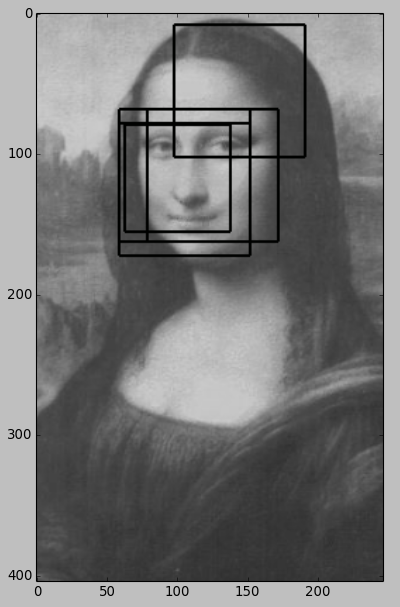
\includegraphics[height = 1.7in, width = 1.5in ]{../figure/overlappedResult.png}
        }
        \subfloat[Detection result after optimalization]
        {
            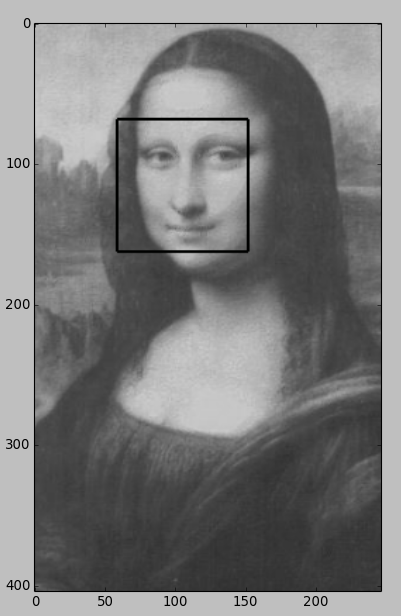
\includegraphics[height = 1.7in, width = 1.5in ]{../figure/afterOptimalization.png}
        }
        \caption{Comparision between two images. overlap\_threshold = 0.1, scale range $\in (0.2, 0.35)$ }
    \end{figure}


%\clearpage
\section{Results}
    Some test on normal images are shown below there.\\

    \begin{figure}[H]
        \centering
        \subfloat[]
        {
            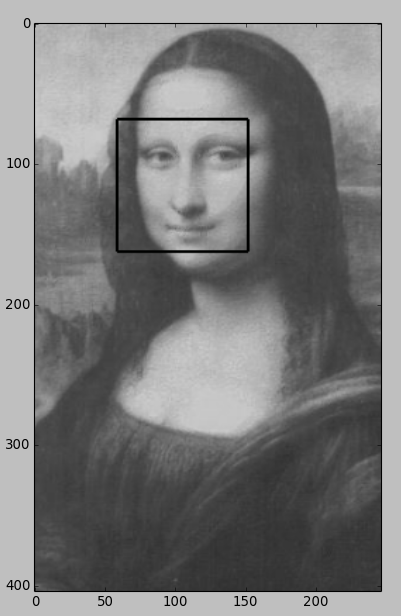
\includegraphics[height = 3.4in, width = 2.7in ]{../figure/afterOptimalization.png}
        }\\
        \subfloat[scale = 0.4, Final\_th = 0.3]
        {
            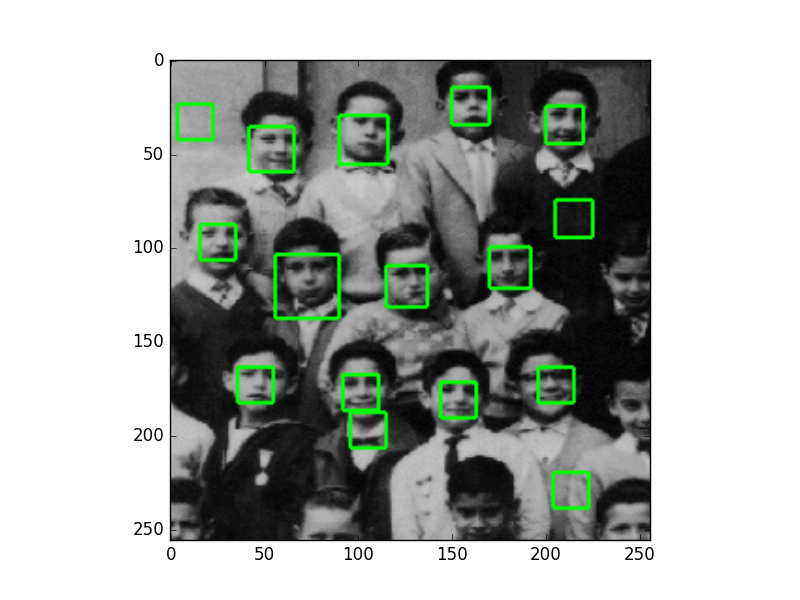
\includegraphics[height = 3.in, width = 3.0in ]{../figure/nens.png}
        }
    \end{figure}


    \clearpage
    \begin{figure}[H]
        \centering
        \subfloat[scale = 0.25]
        {
            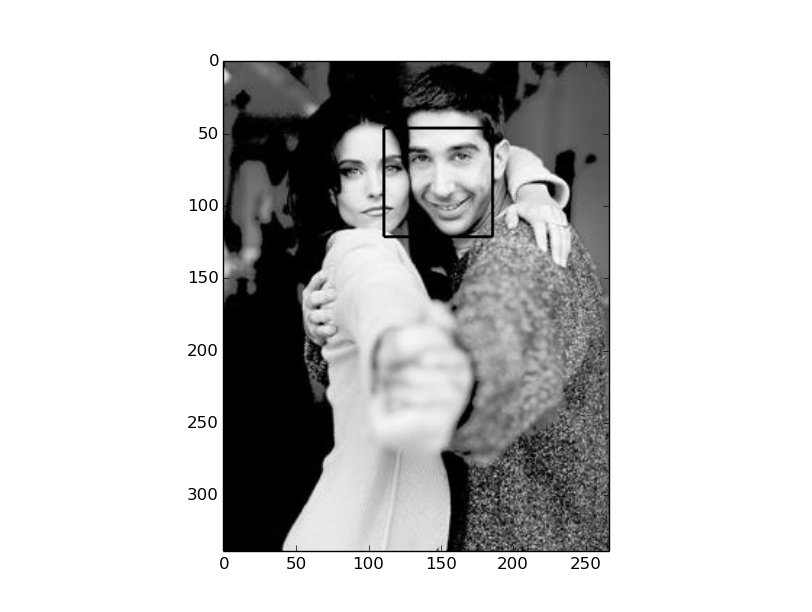
\includegraphics[height = 3.7in, width = 3.7in ]{../figure/ew.png}
        }\\
        \subfloat[scale = 0.3, Final\_th = 1.6, overlap\_th = 0.1]
        {
            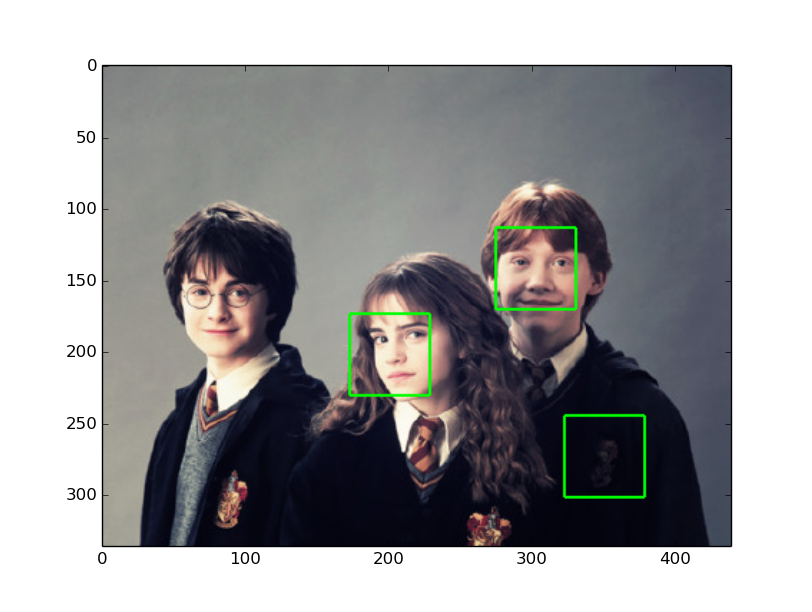
\includegraphics[height = 3.7in, width = 3.7in ]{../figure/harry.png}
        }
    \end{figure}

    \clearpage
    \begin{figure}
        \centering
        \subfloat[scale = 0.2, Final\_th = 1.8, overlap\_th = 0.1]
        {
            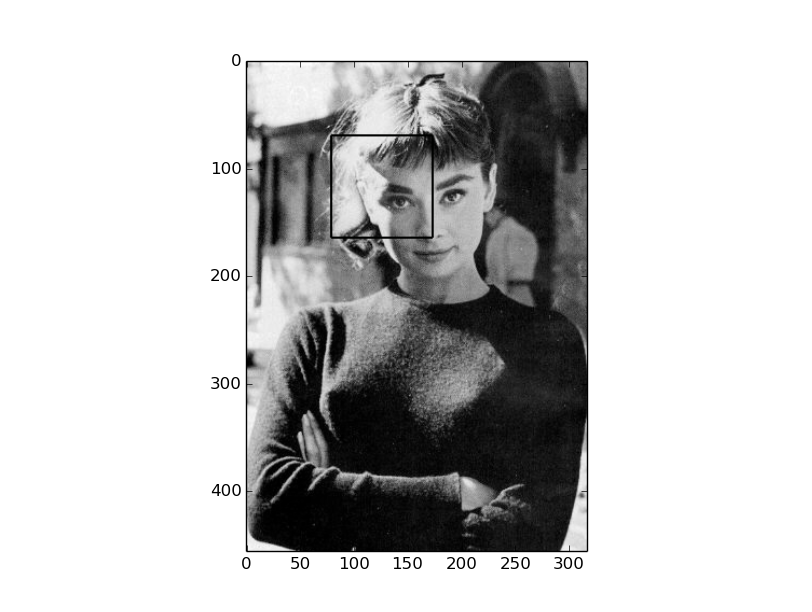
\includegraphics[height = 3.7in, width = 3.7in ]{../figure/herben.png}
        }\\
        \subfloat[scale = 0.25, Final\_th = 1.8, overlap\_th = 0.1]
        {
            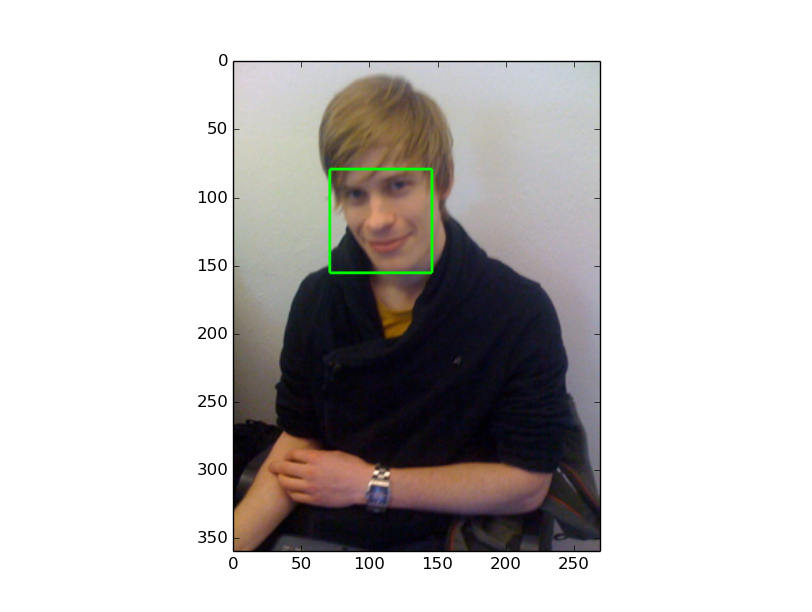
\includegraphics[height = 3.7in, width = 2.7in ]{../figure/boy.png}
        }
        \subfloat[scale = 0.25, Final\_th = 1.8, overlap\_th = 0.1]
        {
            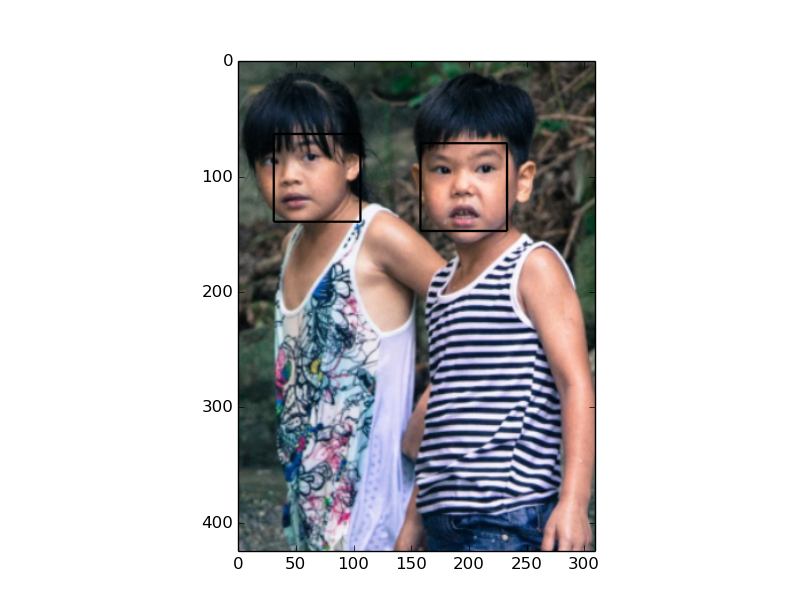
\includegraphics[height = 3.7in, width = 2.7in ]{../figure/gril_and_boy.png}
        }
    \end{figure}

\clearpage
\section{Details of Implementation}
    \begin{figure}[H]
        \centering
        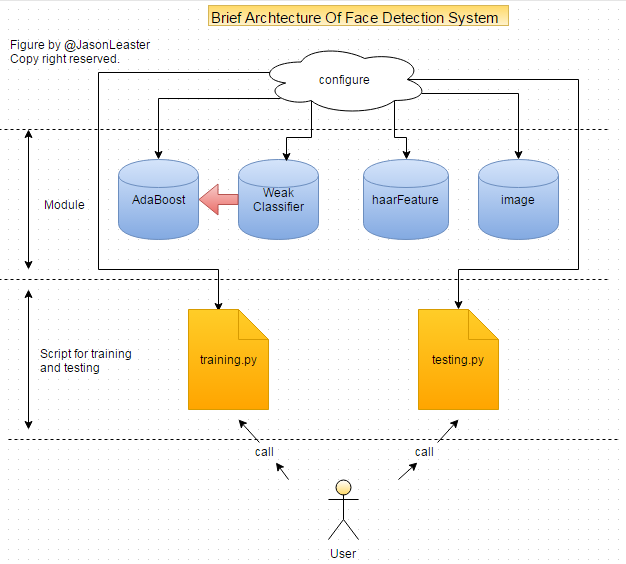
\includegraphics[height = 3.7in, width = 3.7in ]{../figure/architecture.png}
        \caption{scale = 0.2, Final\_th = 1.8, overlap\_th = 0.1}
    \end{figure}

    \begin{figure}[H]
        \centering
        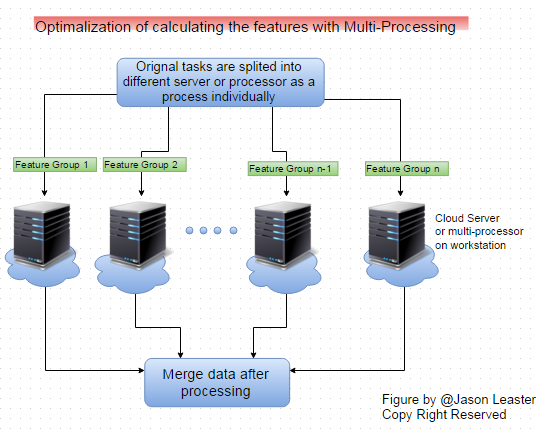
\includegraphics[height = 2.7in, width = 3.7in ]{../figure/concurrent.png}
        \caption{optimalization with Multi-Processing}
    \end{figure}

%\clearpage
%\section{Conclusion}
%
%    Without powerful machine, the final classifier isn't good enough and test result isn't perfect. There still have meanful work to be done to make the detection system more robust.\\
%
%    I wish my work on this application will help someone in the future.\\
%
%\section{Acknowledge}
%
%    Thanks for my parent. I build this project at home day and night. They support me with a good enviornment and paid a lot for me.\\
%
%    I also should say thanks to my friend and teacher(Miss Tang). They give me the chance to try something different in computer vision.\\
%
%    Thanks annabella. When I have no job, it's a dark time for me. She stay with me and encourage me.\\

\clearpage
\vspace*{\fill}
\begin{center}
    \textit{Tell me and I forget, teach me and I may remember, involve me and I learn\\ -- Benjamin Franklin}
\end{center}
\vspace*{\fill}

\clearpage
\bibliographystyle{unsrt}
\bibliography{faceDetection}

\end{document}
